\documentclass{beamer}

\usetheme{Hannover}

\usefonttheme{professionalfonts}
%% \usefonttheme[onlymath]{serif}

\setbeamertemplate{enumerate items}[default]
\setbeamertemplate{navigation symbols}{\insertdocnavigationsymbol}
\setbeamertemplate{section in toc}[default]

\usepackage{polyglossia}

\setmainlanguage[variant=usmax]{english}
\setotherlanguage{spanish}

\usepackage{tikz}

\usepackage{fancyvrb}

\DefineShortVerb{\|}
\DefineVerbatimEnvironment{code}{Verbatim}{frame=lines}

\usepackage{xspace}

%% \usepackage{fontspec}
%% \usepackage{unicode-math}

\usepackage{fontspec}
\usepackage{unicode-math}

\setmathfont{latinmodern-math.otf}

\setmathfont[range={\llparenthesis,\rrparenthesis}]{xits-math.otf}

%%%%%%%%%%%%%%%%%%%%%%%%%%%%%%%%%%%%%%%%%%%%%%%%%%%%%%%%%%%%%%%%%%%%%%%%%%%%%%

\DeclareMathOperator{\obj}{O}
\DeclareMathOperator{\mor}{M}

\DeclareMathOperator{\dom}{dom}
\DeclareMathOperator{\cod}{cod}

\DeclareMathOperator{\id}{id}

\newcommand{\idO}[1]{\natO{\id}{#1}}

\newcommand{\comp}{\ensuremath{\mathrel{\circ}}}

\newcommand{\cat}[1]{\ensuremath{\mathcal{#1}}}

\newcommand{\catbf}[1]{\ensuremath{\mathbf{#1}}\xspace}

\newcommand{\alg}{\catbf{Alg}}
\newcommand{\falg}[1]{\func{#1}\text{-}\alg}
\newcommand{\hask}{\catbf{Hask}}
\newcommand{\set}{\catbf{Set}}

\newcommand{\func}[1]{\ensuremath{\mathsf{#1}}}

\newcommand{\funcO}[1]{\ensuremath{\func{#1}_{\obj}}}
\newcommand{\funcM}[1]{\ensuremath{\func{#1}_{\mor}}}

\newcommand{\nat}[1]{\ensuremath{#1}}

\newcommand{\natO}[2]{\ensuremath{\nat{#1}_{#2}}}

\newcommand{\underscore}{\ensuremath{\underline{\ }}}

\newcommand{\mon}[1]{\func{#1}}

\newcommand{\monM}[2]{\ensuremath{#2^*}}

\DeclareMathOperator{\inmo}{in}

\newcommand{\cata}[1]{\ensuremath{\llparenthesis#1\rrparenthesis}}

\DeclareMathOperator{\zero}{zero}
\DeclareMathOperator{\suc}{succ}

\newcommand{\listof}[1]{\text{List}(#1)}

\DeclareMathOperator{\nil}{nil}
\DeclareMathOperator{\cons}{cons}

\DeclareMathOperator{\fold}{fold}
\DeclareMathOperator{\foldr}{foldr}

\DeclareMathOperator{\add}{add}
\DeclareMathOperator{\mul}{mult}

\DeclareMathOperator{\length}{length}
\DeclareMathOperator{\append}{append}
\DeclareMathOperator{\map}{map}

\SaveVerb{False}|False|
\SaveVerb{fmap f}|fmap f|
\SaveVerb{Functor}|Functor|
\SaveVerb{head}|head|
\SaveVerb{id}|id|
\SaveVerb{Monad}|Monad|
\SaveVerb{Monad'}|Monad'|
\SaveVerb{Monad''}|Monad''|
\SaveVerb{Succ}|Succ|
\SaveVerb{True}|True|
\SaveVerb{Zero}|Zero|
\SaveVerb{()}|()|
\SaveVerb{not}|not|
\SaveVerb{isZero}|isZero|

%%%%%%%%%%%%%%%%%%%%%%%%%%%%%%%%%%%%%%%%%%%%%%%%%%%%%%%%%%%%%%%%%%%%%%%%%%%%%%
%%%%%%%%%%%%%%%%%%%%%%%%%%%%%%%%%%%%%%%%%%%%%%%%%%%%%%%%%%%%%%%%%%%%%%%%%%%%%%
%%%%%%%%%%%%%%%%%%%%%%%%%%%%%%%%%%%%%%%%%%%%%%%%%%%%%%%%%%%%%%%%%%%%%%%%%%%%%%
%%%%%%%%%%%%%%%%%%%%%%%%%%%%%%%%%%%%%%%%%%%%%%%%%%%%%%%%%%%%%%%%%%%%%%%%%%%%%%

\title{Category Theory Applied to Functional Programming}

\subtitle{Systems Engineering Undergraduate Project}

\author[Juan Pedro Villa Isaza]{Juan Pedro Villa Isaza\\
  Supervisor: Andrés Sicard Ramírez}

\institute{EAFIT University}

\date{2014}

\hypersetup{pdfauthor={Juan Pedro Villa Isaza}}

\begin{document}

\frame{\titlepage}

\frame{\frametitle{Contents}\tableofcontents}

%%%%%%%%%%%%%%%%%%%%%%%%%%%%%%%%%%%%%%%%%%%%%%%%%%%%%%%%%%%%%%%%%%%%%%%%%%%%%%
%%%%%%%%%%%%%%%%%%%%%%%%%%%%%%%%%%%%%%%%%%%%%%%%%%%%%%%%%%%%%%%%%%%%%%%%%%%%%%
%%%%%%%%%%%%%%%%%%%%%%%%%%%%%%%%%%%%%%%%%%%%%%%%%%%%%%%%%%%%%%%%%%%%%%%%%%%%%%

\section{Introduction}

%%%%%%%%%%%%%%%%%%%%%%%%%%%%%%%%%%%%%%%%%%%%%%%%%%%%%%%%%%%%%%%%%%%%%%%%%%%%%%

\begin{frame}[label={introduction}]
  \frametitle{Introduction}

  \begin{itemize}
  \item
    Category theory is a branch of mathematics developed in the 1940s.
  \item
    It is a convenient conceptual framework based on:
    \begin{itemize}
    \item
      Categories
    \item
      Functors
    \item
      Natural transformations
    \end{itemize}
  \end{itemize}

\end{frame}

%%%%%%%%%%%%%%%%%%%%%%%%%%%%%%%%%%%%%%%%%%%%%%%%%%%%%%%%%%%%%%%%%%%%%%%%%%%%%%

\begin{frame}
  \frametitle{Introduction}

  \begin{itemize}
  \item
    Category theory occupies a central position in:
    \begin{itemize}
    \item
      Computer science
      \begin{itemize}
      \item
        Functional programming
      \end{itemize}
    \end{itemize}
  \item
    Several concepts of functional programming languages are based on
    concepts of category theory:
    \begin{itemize}
    \item
      Functors
    \item
      Monads
    \item
      ...
    \end{itemize}
  \end{itemize}

\end{frame}

%%%%%%%%%%%%%%%%%%%%%%%%%%%%%%%%%%%%%%%%%%%%%%%%%%%%%%%%%%%%%%%%%%%%%%%%%%%%%%
%%%%%%%%%%%%%%%%%%%%%%%%%%%%%%%%%%%%%%%%%%%%%%%%%%%%%%%%%%%%%%%%%%%%%%%%%%%%%%

\subsection[Summary]{Summary of the Project}

%%%%%%%%%%%%%%%%%%%%%%%%%%%%%%%%%%%%%%%%%%%%%%%%%%%%%%%%%%%%%%%%%%%%%%%%%%%%%%

\begin{frame}
  \frametitle{Introduction}
  \framesubtitle{Summary of the Project}

  We examine functional programming through category theory.

\end{frame}

%%%%%%%%%%%%%%%%%%%%%%%%%%%%%%%%%%%%%%%%%%%%%%%%%%%%%%%%%%%%%%%%%%%%%%%%%%%%%%

\begin{frame}[label={aim}]
  \frametitle{Introduction}
  \framesubtitle{Summary of the Project}

  \begin{block}{Aim}
    \begin{itemize}
    \item
      To study some of the applications of category theory to
      functional programming.
    \item
      In the context of:
      \begin{itemize}
      \item
        Haskell
      \item
        Agda
      \end{itemize}
    \end{itemize}
  \end{block}

\end{frame}

%%%%%%%%%%%%%%%%%%%%%%%%%%%%%%%%%%%%%%%%%%%%%%%%%%%%%%%%%%%%%%%%%%%%%%%%%%%%%%

\begin{frame}[label={objectives}]
  \frametitle{Introduction}
  \framesubtitle{Summary of the Project}

  \begin{block}{Objectives}
    \begin{itemize}
    \item
      To describe and explain the concepts of category theory needed
      for conceptualizing and better understanding:
      \begin{enumerate}
      \item
        Functors
      \item
        Parametrically polymorphic functions
      \item
        Monads
      \item
        Algebraic data types
      \end{enumerate}
    \end{itemize}
  \end{block}

\end{frame}

%%%%%%%%%%%%%%%%%%%%%%%%%%%%%%%%%%%%%%%%%%%%%%%%%%%%%%%%%%%%%%%%%%%%%%%%%%%%%%
%%%%%%%%%%%%%%%%%%%%%%%%%%%%%%%%%%%%%%%%%%%%%%%%%%%%%%%%%%%%%%%%%%%%%%%%%%%%%%

\subsection[Overview]{Overview of the Project}

%%%%%%%%%%%%%%%%%%%%%%%%%%%%%%%%%%%%%%%%%%%%%%%%%%%%%%%%%%%%%%%%%%%%%%%%%%%%%%

\begin{frame}[label={overview}]
  \frametitle{Introduction}
  \framesubtitle{Overview of the Project}

  \begin{columns}[onlytextwidth,c]
    \begin{column}{.8\textwidth}
      \begin{block}{Chapters}
        \begin{itemize}
        \item Chapter 2 (Categories)
        \item Chapter 3 (Constructions)
        \item Chapter 4 (Functors)
        \item Chapter 5 (Natural Transformations)
        \item Chapter 6 (Monads and Kleisli Triples)
        \item Chapter 7 (Algebras and Initial Algebras)
        \end{itemize}
      \end{block}
    \end{column}
    \begin{column}{.2\textwidth}
      \begin{center}
        \begin{tikzpicture}[auto]
          \node (2)                    {2};
          \node (3) [below of=2]       {3};
          \node (4) [below of=3]       {4};
          \node (5) [below left of=4]  {5};
          \node (6) [below of=5]       {6};
          \node (7) [below right of=4] {7};
          \node (c) [right of=3]       {};

          \draw [->,dashed] (2) to (3);
          \draw [->,dashed] (3) to (4);
          \draw [->]        (4) to (5);
          \draw [->]        (5) to (6);
          \draw [->]        (4) to (7);
          \draw [->]        (2) .. controls (c) .. (4);
        \end{tikzpicture}
      \end{center}
    \end{column}
  \end{columns}

\end{frame}

%%%%%%%%%%%%%%%%%%%%%%%%%%%%%%%%%%%%%%%%%%%%%%%%%%%%%%%%%%%%%%%%%%%%%%%%%%%%%%

\begin{frame}[label={chap:categories}]
  \frametitle{Introduction}
  \framesubtitle{Overview of the Project}

  \begin{columns}[onlytextwidth,t]
    \begin{column}{\textwidth}
      \begin{block}{Chapters}
        \begin{itemize}
        \item Chapter 2 (Categories)
        \end{itemize}
      \end{block}
    \end{column}
  \end{columns}
  \begin{columns}[onlytextwidth,t]
    \begin{column}{.5\textwidth}
      \begin{block}{Category theory}
        \begin{itemize}
        \item Categories
        \item Commutative diagrams
        \end{itemize}
      \end{block}
    \end{column}
    \begin{column}{.5\textwidth}
      \begin{block}{Functional programming}
        \begin{itemize}
        \item A category for Haskell
        \item A category for Agda
        \end{itemize}
      \end{block}
    \end{column}
  \end{columns}
  \begin{columns}[onlytextwidth,t]
    \begin{column}{\textwidth}
      \begin{block}{Aim and objectives}
        \begin{itemize}
        \item All
        \end{itemize}
      \end{block}
    \end{column}
  \end{columns}

\end{frame}

%%%%%%%%%%%%%%%%%%%%%%%%%%%%%%%%%%%%%%%%%%%%%%%%%%%%%%%%%%%%%%%%%%%%%%%%%%%%%%

\begin{frame}[label={chap:constructions}]
  \frametitle{Introduction}
  \framesubtitle{Overview of the Project}

  \begin{columns}[onlytextwidth,t]
    \begin{column}{\textwidth}
      \begin{block}{Chapters}
        \begin{itemize}
        \item Chapter 3 (Constructions)
        \end{itemize}
      \end{block}
    \end{column}
  \end{columns}
  \begin{columns}[onlytextwidth,t]
    \begin{column}{.5\textwidth}
      \begin{block}{Category theory}
        \begin{itemize}
        \item Isomorphisms
        \item Initial and terminal objects
        \item Products and coproducts
        \end{itemize}
      \end{block}
    \end{column}
    \begin{column}{.5\textwidth}
      \begin{block}{Functional programming}
        \begin{itemize}
        \item Empty and unit types in Haskell and Agda
        \item Products and sums in Haskell and Agda
        \end{itemize}
      \end{block}
    \end{column}
  \end{columns}
  \begin{columns}[onlytextwidth,t]
    \begin{column}{\textwidth}
      \begin{block}{Aim and objectives}
        \begin{itemize}
        \item Auxiliary
        \end{itemize}
      \end{block}
    \end{column}
  \end{columns}

\end{frame}

%%%%%%%%%%%%%%%%%%%%%%%%%%%%%%%%%%%%%%%%%%%%%%%%%%%%%%%%%%%%%%%%%%%%%%%%%%%%%%

\begin{frame}[label={chap:functors}]
  \frametitle{Introduction}
  \framesubtitle{Overview of the Project}

  \begin{columns}[onlytextwidth,t]
    \begin{column}{\textwidth}
      \begin{block}{Chapters}
        \begin{itemize}
        \item Chapter 4 (Functors)
        \end{itemize}
      \end{block}
    \end{column}
  \end{columns}
  \begin{columns}[onlytextwidth,t]
    \begin{column}{.5\textwidth}
      \begin{block}{Category theory}
        \begin{itemize}
        \item Functors
        \item Endofunctors
        \end{itemize}
      \end{block}
    \end{column}
    \begin{column}{.5\textwidth}
      \begin{block}{Functional programming}
        \begin{itemize}
        \item Functors in Haskell
        \item Functors in Agda
        \end{itemize}
      \end{block}
    \end{column}
  \end{columns}
  \begin{columns}[onlytextwidth,t]
    \begin{column}{\textwidth}
      \begin{block}{Aim and objectives}
        \begin{itemize}
        \item Objective 1 (Functors)
        \end{itemize}
      \end{block}
    \end{column}
  \end{columns}

\end{frame}

%%%%%%%%%%%%%%%%%%%%%%%%%%%%%%%%%%%%%%%%%%%%%%%%%%%%%%%%%%%%%%%%%%%%%%%%%%%%%%

\begin{frame}[label={chap:naturals}]
  \frametitle{Introduction}
  \framesubtitle{Overview of the Project}

  \begin{columns}[onlytextwidth,t]
    \begin{column}{\textwidth}
      \begin{block}{Chapters}
        \begin{itemize}
        \item Chapter 5 (Natural Transformations)
        \end{itemize}
      \end{block}
    \end{column}
  \end{columns}
  \begin{columns}[onlytextwidth,t]
    \begin{column}{.5\textwidth}
      \begin{block}{Category theory}
        \begin{itemize}
        \item Natural transformations
        \end{itemize}
      \end{block}
    \end{column}
    \begin{column}{.5\textwidth}
      \begin{block}{Functional programming}
        \begin{itemize}
        \item Parametrically polymorphic functions in Haskell
        \end{itemize}
      \end{block}
    \end{column}
  \end{columns}
  \begin{columns}[onlytextwidth,t]
    \begin{column}{\textwidth}
      \begin{block}{Aim and objectives}
        \begin{itemize}
        \item Objective 2 (Parametrically polymorphic functions)
        \end{itemize}
      \end{block}
    \end{column}
  \end{columns}

\end{frame}

%%%%%%%%%%%%%%%%%%%%%%%%%%%%%%%%%%%%%%%%%%%%%%%%%%%%%%%%%%%%%%%%%%%%%%%%%%%%%%

\begin{frame}[label={chap:monads}]
  \frametitle{Introduction}
  \framesubtitle{Overview of the Project}

  \begin{columns}[onlytextwidth,t]
    \begin{column}{\textwidth}
      \begin{block}{Chapters}
        \begin{itemize}
        \item Chapter 6 (Monads and Kleisli Triples)
        \end{itemize}
      \end{block}
    \end{column}
  \end{columns}
  \begin{columns}[onlytextwidth,t]
    \begin{column}{.5\textwidth}
      \begin{block}{Category theory}
        \begin{itemize}
        \item Monads
        \item Kleisli triples
        \item Monads $=$ Kleisli triples
        \end{itemize}
      \end{block}
    \end{column}
    \begin{column}{.5\textwidth}
      \begin{block}{Functional programming}
        \begin{itemize}
        \item Monads in Haskell
        \item Monads in Agda
        \end{itemize}
      \end{block}
    \end{column}
  \end{columns}
  \begin{columns}[onlytextwidth,t]
    \begin{column}{\textwidth}
      \begin{block}{Aim and objectives}
        \begin{itemize}
        \item Objective 3 (Monads)
        \end{itemize}
      \end{block}
    \end{column}
  \end{columns}

\end{frame}

%%%%%%%%%%%%%%%%%%%%%%%%%%%%%%%%%%%%%%%%%%%%%%%%%%%%%%%%%%%%%%%%%%%%%%%%%%%%%%

\begin{frame}[label={chap:algebras}]
  \frametitle{Introduction}
  \framesubtitle{Overview of the Project}

  \begin{columns}[onlytextwidth,t]
    \begin{column}{\textwidth}
      \begin{block}{Chapters}
        \begin{itemize}
        \item Chapter 7 (Algebras and Initial Algebras)
        \end{itemize}
      \end{block}
    \end{column}
  \end{columns}
  \begin{columns}[onlytextwidth,t]
    \begin{column}{.5\textwidth}
      \begin{block}{Category theory}
        \begin{itemize}
        \item Algebras and initial algebras over endofunctors
        \end{itemize}
      \end{block}
    \end{column}
    \begin{column}{.5\textwidth}
      \begin{block}{Functional programming}
        \begin{itemize}
        \item Algebraic data types and folds in Haskell
        \end{itemize}
      \end{block}
    \end{column}
  \end{columns}
  \begin{columns}[onlytextwidth,t]
    \begin{column}{\textwidth}
      \begin{block}{Aim and objectives}
        \begin{itemize}
        \item Objective 4 (Algebraic data types)
        \end{itemize}
      \end{block}
    \end{column}
  \end{columns}

\end{frame}

%%%%%%%%%%%%%%%%%%%%%%%%%%%%%%%%%%%%%%%%%%%%%%%%%%%%%%%%%%%%%%%%%%%%%%%%%%%%%%

\begin{frame}[label={overview-presentation}]
  \frametitle{Introduction}
  \framesubtitle{Overview of the Presentation}

  \begin{columns}[onlytextwidth,c]
    \begin{column}{.8\textwidth}
      \begin{block}{Chapters}
        \begin{itemize}
        \item \alert{Chapter 2 (Categories)}
        \item Chapter 3 (Constructions)
        \item \alert{Chapter 4 (Functors)}
        \item Chapter 5 (Natural Transformations)
        \item Chapter 6 (Monads and Kleisli Triples)
        \item Chapter 7 (Algebras and Initial Algebras)
        \end{itemize}
      \end{block}
    \end{column}
    \begin{column}{.2\textwidth}
      \begin{center}
        \begin{tikzpicture}[auto]
          \node (2)                    {\alert{2}};
          \node (3) [below of=2]       {3};
          \node (4) [below of=3]       {\alert{4}};
          \node (5) [below left of=4]  {5};
          \node (6) [below of=5]       {6};
          \node (7) [below right of=4] {7};
          \node (c) [right of=3]       {};

          \draw [->,dashed] (2) to (3);
          \draw [->,dashed] (3) to (4);
          \draw [->]        (4) to (5);
          \draw [->]        (5) to (6);
          \draw [->]        (4) to (7);
          \draw [->]        (2) .. controls (c) .. (4);
        \end{tikzpicture}
      \end{center}
    \end{column}
  \end{columns}

\end{frame}

%%%%%%%%%%%%%%%%%%%%%%%%%%%%%%%%%%%%%%%%%%%%%%%%%%%%%%%%%%%%%%%%%%%%%%%%%%%%%%
%%%%%%%%%%%%%%%%%%%%%%%%%%%%%%%%%%%%%%%%%%%%%%%%%%%%%%%%%%%%%%%%%%%%%%%%%%%%%%
%%%%%%%%%%%%%%%%%%%%%%%%%%%%%%%%%%%%%%%%%%%%%%%%%%%%%%%%%%%%%%%%%%%%%%%%%%%%%%

\section{Categories}

%%%%%%%%%%%%%%%%%%%%%%%%%%%%%%%%%%%%%%%%%%%%%%%%%%%%%%%%%%%%%%%%%%%%%%%%%%%%%%

\begin{frame}[label={def:category}]
  \frametitle{Categories}

  \begin{definition}[Category]
    A category \cat{C} consists of:
    \begin{itemize}
    \item
      Objects $a$, $b$, $c$, ...
    \item
      Morphisms $f: a \to b$, $g: b \to c$, ...
    \item
      Identity morphisms $\idO{a}: a \to a$, $\idO{b}: b \to b$,
      $\idO{c}: c \to c$, ...
    \item
      Composite morphisms $g \comp f: a \to c$, ...
    \end{itemize}
    Such that:
    \begin{itemize}
    \item
      Associativity: $h \comp (g \comp f) = (h \comp g) \comp f$
    \item
      Identity: $\idO{b} \comp f = f = f \comp \idO{a}$
    \end{itemize}
  \end{definition}

\end{frame}

%%%%%%%%%%%%%%%%%%%%%%%%%%%%%%%%%%%%%%%%%%%%%%%%%%%%%%%%%%%%%%%%%%%%%%%%%%%%%%

\begin{frame}
  \frametitle{Categories}

  \begin{definition}[Category]
    \begin{itemize}
    \item
      Associativity: $h \comp (g \comp f) = (h \comp g) \comp f$
    \end{itemize}
  \end{definition}
  \begin{center}
    \begin{tikzpicture}[auto,node distance=3cm]
      \node (a)              {$a$};
      \node (b) [right of=a] {$b$};
      \node (c) [below of=b] {$c$};
      \node (d) [right of=c] {$d$};

      \draw [->] (a) to node        {$f$}         (b);
      \draw [->] (b) to node        {$g$}         (c);
      \draw [->] (c) to node [swap] {$h$}         (d);

      \draw [->] (a) to node [swap] {$g \comp f$} (c);
      \draw [->] (b) to node        {$h \comp g$} (d);
    \end{tikzpicture}
  \end{center}

\end{frame}

%%%%%%%%%%%%%%%%%%%%%%%%%%%%%%%%%%%%%%%%%%%%%%%%%%%%%%%%%%%%%%%%%%%%%%%%%%%%%%

\begin{frame}
  \frametitle{Categories}

  \begin{definition}[Category]
    \begin{itemize}
    \item
      Identity: $\idO{b} \comp f = f = f \comp \idO{a}$
    \end{itemize}
  \end{definition}
  \begin{center}
    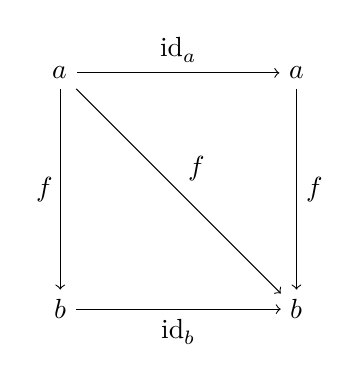
\begin{tikzpicture}[auto,node distance=3cm]
      \node (a1)               {$a$};
      \node (a2) [right of=a1] {$a$};
      \node (b1) [below of=a1] {$b$};
      \node (b2) [right of=b1] {$b$};

      \draw [->] (a1) to node        {$\idO{a}$} (a2);
      \draw [->] (b1) to node [swap] {$\idO{b}$} (b2);

      \draw [->] (a1) to node [swap] {$f$}       (b1);
      \draw [->] (a1) to node        {$f$}       (b2);
      \draw [->] (a2) to node        {$f$}       (b2);
    \end{tikzpicture}
  \end{center}

\end{frame}

%%%%%%%%%%%%%%%%%%%%%%%%%%%%%%%%%%%%%%%%%%%%%%%%%%%%%%%%%%%%%%%%%%%%%%%%%%%%%%

\begin{frame}[label={ex:set}]
  \frametitle{Categories}

  \begin{example}
    \set is the category of sets and functions.
    \begin{itemize}
    \item
      Objects: Sets $A$, $B$, $C$, ...
    \item
      Morphisms: Functions $f: A \to B$, $g: B \to C$, ...
    \item
      Identities: $\idO{A}: A \to A$ such that $\idO{A}(x) = x$, ...
    \item
      Composites: $g \comp f: A \to C$ such that $(g \comp f)(x) =
      g(f(x))$, ...
    \end{itemize}
  \end{example}
  \vfill\hfill\hyperlink{re:foundations}{\beamergotobutton{}}

\end{frame}

%%%%%%%%%%%%%%%%%%%%%%%%%%%%%%%%%%%%%%%%%%%%%%%%%%%%%%%%%%%%%%%%%%%%%%%%%%%%%%
%%%%%%%%%%%%%%%%%%%%%%%%%%%%%%%%%%%%%%%%%%%%%%%%%%%%%%%%%%%%%%%%%%%%%%%%%%%%%%

\subsection{A Category for Haskell}

%%%%%%%%%%%%%%%%%%%%%%%%%%%%%%%%%%%%%%%%%%%%%%%%%%%%%%%%%%%%%%%%%%%%%%%%%%%%%%

\begin{frame}[fragile]
  \frametitle{Categories}
  \framesubtitle{A Category for Haskell}

  \begin{center}
    \begin{tikzpicture}[auto,node distance=4cm]
      \node (bool) at (0,0)  {|Bool|};
      \node (nat)  at (5,1)  {|Nat|};
      \node (unit) at (3,-2) {|()|};

      \draw [->] (unit) to node [swap] {\UseVerb{False}} (bool);
      \draw [->] (unit) to node        {\UseVerb{True}}  (bool);

      \draw [->] (unit) to              node [swap] {\UseVerb{Zero}} (nat);
      \draw [->] (nat)  to [loop above] node        {\UseVerb{Succ}} (nat);

      \draw [->] (unit) to [loop below] node {\UseVerb{()}} (unit);

      \draw [->] (bool) to [loop left]  node {\UseVerb{id}} (bool);
      \draw [->] (nat)  to [loop right] node {\UseVerb{id}} (nat);
      \draw [->] (unit) to [loop right] node {\UseVerb{id}} (unit);

      \draw [->] (bool) to [loop above] node        {\UseVerb{not}}    (bool);
      \draw [->] (nat)  to              node [swap] {\UseVerb{isZero}} (bool);
    \end{tikzpicture}
  \end{center}

\end{frame}

%%%%%%%%%%%%%%%%%%%%%%%%%%%%%%%%%%%%%%%%%%%%%%%%%%%%%%%%%%%%%%%%%%%%%%%%%%%%%%

\begin{frame}[fragile,label={ex:hask}]
  \frametitle{Categories}
  \framesubtitle{A Category for Haskell}

  \begin{example}
    \hask is the category of Haskell types and functions.
    \begin{itemize}
    \item
      Objects: Haskell types with kind |*|, like |Bool|:
      \begin{code}
data Bool = False | True
      \end{code}
    \item
      Morphisms: Haskell functions, like |not|:
      \begin{code}
not :: Bool -> Bool -> Bool
not False = True
not True  = False
      \end{code}
    \end{itemize}
  \end{example}
  \vfill\hfill\hyperlink{re:hask}{\beamergotobutton{}}

\end{frame}

%%%%%%%%%%%%%%%%%%%%%%%%%%%%%%%%%%%%%%%%%%%%%%%%%%%%%%%%%%%%%%%%%%%%%%%%%%%%%%

\begin{frame}[fragile]
  \frametitle{Categories}
  \framesubtitle{A Category for Haskell}

  \begin{example}
    \hask is the category of Haskell types and functions.
    \begin{itemize}
    \item
      Identities:
      \begin{code}
id :: a -> a
id x = x
      \end{code}
    \item
      Composites:
      \begin{code}
(.) :: (b -> c) -> (a -> b) -> a -> c
(g . f) x = g (f x)
      \end{code}
    \end{itemize}
  \end{example}

\end{frame}

%%%%%%%%%%%%%%%%%%%%%%%%%%%%%%%%%%%%%%%%%%%%%%%%%%%%%%%%%%%%%%%%%%%%%%%%%%%%%%
%%%%%%%%%%%%%%%%%%%%%%%%%%%%%%%%%%%%%%%%%%%%%%%%%%%%%%%%%%%%%%%%%%%%%%%%%%%%%%
%%%%%%%%%%%%%%%%%%%%%%%%%%%%%%%%%%%%%%%%%%%%%%%%%%%%%%%%%%%%%%%%%%%%%%%%%%%%%%

\section{Functors}

%%%%%%%%%%%%%%%%%%%%%%%%%%%%%%%%%%%%%%%%%%%%%%%%%%%%%%%%%%%%%%%%%%%%%%%%%%%%%%

\begin{frame}
  \frametitle{Functors}

  \begin{quote}
    \emph{Category} has been defined in order to be able to define
    \emph{functor}...
  \end{quote}
  \hfill ---Saunders Mac Lane

\end{frame}

%%%%%%%%%%%%%%%%%%%%%%%%%%%%%%%%%%%%%%%%%%%%%%%%%%%%%%%%%%%%%%%%%%%%%%%%%%%%%%

\begin{frame}[label={def:functor}]
  \frametitle{Functors}

  \begin{definition}[Functor]
    \begin{itemize}
    \item
      Let \cat{C} and \cat{D} be categories.
    \item
      A functor $\func{F}: \cat{C} \to \cat{D}$ assigns:
      \begin{itemize}
      \item
        To each object $a$ in \cat{C},\\ an object $\funcO{F}(a)$ in
        \cat{D}.
      \item
        To each morphism $f: a \to b$ in \cat{C},\\ a morphism
        $\funcM{F}(f): \funcO{F}(a) \to \funcO{F}(b)$ in \cat{D}.
      \end{itemize}
    \item
      Such that:
      \begin{itemize}
      \item
        $\funcM{F}(\idO{a}) = \idO{\funcO{F}(a)}$
      \item
        $\funcM{F}(g \comp f) = \funcM{F}(g) \comp \funcM{F}(f)$
      \end{itemize}
    \end{itemize}
  \end{definition}

\end{frame}

%%%%%%%%%%%%%%%%%%%%%%%%%%%%%%%%%%%%%%%%%%%%%%%%%%%%%%%%%%%%%%%%%%%%%%%%%%%%%%

\begin{frame}[label={def:endofunctor}]
  \frametitle{Functors}

  \begin{definition}[Endofunctor]
    \begin{itemize}
    \item
      Let \cat{C} be a category.
    \item
      A functor $\func{F}: \cat{C} \to \cat{C}$ is called an
      endofunctor.
    \end{itemize}
  \end{definition}

\end{frame}

%%%%%%%%%%%%%%%%%%%%%%%%%%%%%%%%%%%%%%%%%%%%%%%%%%%%%%%%%%%%%%%%%%%%%%%%%%%%%%
%%%%%%%%%%%%%%%%%%%%%%%%%%%%%%%%%%%%%%%%%%%%%%%%%%%%%%%%%%%%%%%%%%%%%%%%%%%%%%

\subsection{Functors in Haskell}

%%%%%%%%%%%%%%%%%%%%%%%%%%%%%%%%%%%%%%%%%%%%%%%%%%%%%%%%%%%%%%%%%%%%%%%%%%%%%%

\begin{frame}[fragile]
  \frametitle{Functors}
  \framesubtitle{Functors in Haskell}

  \begin{definition}[\UseVerb{Functor}]
    \begin{code}
class Functor f where
  fmap :: (a -> b) -> f a -> f b
    \end{code}
  \end{definition}

\end{frame}

%%%%%%%%%%%%%%%%%%%%%%%%%%%%%%%%%%%%%%%%%%%%%%%%%%%%%%%%%%%%%%%%%%%%%%%%%%%%%%

\begin{frame}[fragile]
  \frametitle{Functors}
  \framesubtitle{Functors in Haskell}

  \begin{definition}[\UseVerb{Functor}]
    A |Functor| is an endofunctor in \hask:
    \begin{code}
class Functor (f :: * -> *) where
  fmap :: (a -> b) -> (f a -> f b)
    \end{code}
    Such that:
    \begin{code}
fmap id      = id
fmap (g . f) = fmap g . fmap f
    \end{code}
  \end{definition}

\end{frame}

%%%%%%%%%%%%%%%%%%%%%%%%%%%%%%%%%%%%%%%%%%%%%%%%%%%%%%%%%%%%%%%%%%%%%%%%%%%%%%

\begin{frame}[fragile]
  \frametitle{Functors}
  \framesubtitle{Functors in Haskell}

  \begin{example}
    \begin{code}
data Maybe a = Nothing | Just a

instance Functor Maybe where
  fmap :: (a -> b) -> Maybe a -> Maybe b
  fmap _ Nothing  = Nothing
  fmap f (Just x) = Just (f x)
    \end{code}
  \end{example}

\end{frame}

%%%%%%%%%%%%%%%%%%%%%%%%%%%%%%%%%%%%%%%%%%%%%%%%%%%%%%%%%%%%%%%%%%%%%%%%%%%%%%

\begin{frame}[fragile]
  \frametitle{Functors}
  \framesubtitle{Functors in Haskell}

  \begin{example}
    \begin{code}
data [] a = [] | a : [a]

instance Functor [] where
  fmap :: (a -> b) -> [a] -> [b]
  fmap _ []     = []
  fmap f (x:xs) = f x : fmap f xs
    \end{code}
  \end{example}

\end{frame}

%%%%%%%%%%%%%%%%%%%%%%%%%%%%%%%%%%%%%%%%%%%%%%%%%%%%%%%%%%%%%%%%%%%%%%%%%%%%%%

\begin{frame}[fragile]
  \frametitle{Functors}
  \framesubtitle{Functors in Haskell}

  \begin{alertblock}{Example?}
    \begin{code}
data [] a = [] | a : [a]

instance Functor [] where
  fmap :: (a -> b) -> [a] -> [b]
  fmap _ []     = []
  fmap f (x:xs) = f x : f x : fmap f xs
    \end{code}
  \end{alertblock}

\end{frame}

%%%%%%%%%%%%%%%%%%%%%%%%%%%%%%%%%%%%%%%%%%%%%%%%%%%%%%%%%%%%%%%%%%%%%%%%%%%%%%
%%%%%%%%%%%%%%%%%%%%%%%%%%%%%%%%%%%%%%%%%%%%%%%%%%%%%%%%%%%%%%%%%%%%%%%%%%%%%%
%%%%%%%%%%%%%%%%%%%%%%%%%%%%%%%%%%%%%%%%%%%%%%%%%%%%%%%%%%%%%%%%%%%%%%%%%%%%%%

\section{Conclusions}

%%%%%%%%%%%%%%%%%%%%%%%%%%%%%%%%%%%%%%%%%%%%%%%%%%%%%%%%%%%%%%%%%%%%%%%%%%%%%%

\begin{frame}
  \frametitle{Conclusions}

  \begin{itemize}
  \item
    We did not cover all of category theory.
  \end{itemize}
  \begin{itemize}
  \item
    But we did cover categories and functors:
    \begin{itemize}
    \item
      An appropriate starting point for the study of category theory
      applied to functional programming.
    \item
      An overview of the project.
    \end{itemize}
  \end{itemize}

\end{frame}

%%%%%%%%%%%%%%%%%%%%%%%%%%%%%%%%%%%%%%%%%%%%%%%%%%%%%%%%%%%%%%%%%%%%%%%%%%%%%%

\begin{frame}
  \frametitle{Conclusions}

  \begin{itemize}
  \item
    Studying category theory may not be necessary for functional
    programming.
  \end{itemize}
  \begin{itemize}
  \item
    But it is useful for:
    \begin{itemize}
    \item
      Better understanding functional programming.
    \item
      Becoming a better functional programmer.
    \end{itemize}
  \end{itemize}

\end{frame}

%%%%%%%%%%%%%%%%%%%%%%%%%%%%%%%%%%%%%%%%%%%%%%%%%%%%%%%%%%%%%%%%%%%%%%%%%%%%%%

\begin{frame}
  \frametitle{Conclusions}

  \begin{itemize}
  \item
    Difficult? At first.
  \end{itemize}
  \vfill
  \begin{quote}
    One does not so much learn category theory as absorb it over a
    period of time.
  \end{quote}
  \hfill ---Richard Bird and Oege de Moor \vfill
  \begin{itemize}
  \item
    Definitely worth it.
  \end{itemize}

\end{frame}

%%%%%%%%%%%%%%%%%%%%%%%%%%%%%%%%%%%%%%%%%%%%%%%%%%%%%%%%%%%%%%%%%%%%%%%%%%%%%%
%%%%%%%%%%%%%%%%%%%%%%%%%%%%%%%%%%%%%%%%%%%%%%%%%%%%%%%%%%%%%%%%%%%%%%%%%%%%%%

\subsection{Future Work}

%%%%%%%%%%%%%%%%%%%%%%%%%%%%%%%%%%%%%%%%%%%%%%%%%%%%%%%%%%%%%%%%%%%%%%%%%%%%%%

\begin{frame}[fragile,label={future-work}]
  \frametitle{Conclusions}
  \framesubtitle{Future Work}

  \begin{itemize}
  \item
    Adjoints, which ``arise everywhere.''
  \end{itemize}
  \begin{itemize}
  \item
    Applicative functors:
    \begin{itemize}
    \item
      Monoidal categories and functors.
    \item
      Haskell 2014 |Applicative => Monad| proposal.
    \end{itemize}
  \end{itemize}

\end{frame}

%%%%%%%%%%%%%%%%%%%%%%%%%%%%%%%%%%%%%%%%%%%%%%%%%%%%%%%%%%%%%%%%%%%%%%%%%%%%%%

\begin{frame}[fragile]
  \frametitle{Conclusions}
  \framesubtitle{Future Work}

  \begin{itemize}
  \item
    Categories
    \begin{itemize}
    \item
      The |Category| type class.
    \end{itemize}
  \end{itemize}
  \begin{itemize}
  \item
    Folds.
    \begin{itemize}
    \item
      The |Foldable| type class.
    \item
      The |Traversable| type class.
    \end{itemize}
  \end{itemize}
  \begin{itemize}
  \item
    Monoids, a ``fundamental notion of category theory''.
    \begin{itemize}
    \item
      The |Monoid| type class.
    \end{itemize}
  \end{itemize}

\end{frame}

%%%%%%%%%%%%%%%%%%%%%%%%%%%%%%%%%%%%%%%%%%%%%%%%%%%%%%%%%%%%%%%%%%%%%%%%%%%%%%
%%%%%%%%%%%%%%%%%%%%%%%%%%%%%%%%%%%%%%%%%%%%%%%%%%%%%%%%%%%%%%%%%%%%%%%%%%%%%%
%%%%%%%%%%%%%%%%%%%%%%%%%%%%%%%%%%%%%%%%%%%%%%%%%%%%%%%%%%%%%%%%%%%%%%%%%%%%%%

\section*{Bibliography}

%%%%%%%%%%%%%%%%%%%%%%%%%%%%%%%%%%%%%%%%%%%%%%%%%%%%%%%%%%%%%%%%%%%%%%%%%%%%%%

\begin{frame}
  \frametitle{Bibliography}
  \framesubtitle{Category Theory}

  \begin{thebibliography}{Mac Lane 1998}
  \setbeamertemplate{bibliography item}[book]
  \bibitem[Awodey 2010]{awodey-2010}
    Awodey, Steve (2010).
    \newblock \emph{Category Theory}.
    \newblock 2nd ed. Vol. 52. Oxford Logic Guides.
    \newblock Oxford University Press.
  \setbeamertemplate{bibliography item}[book]
  \bibitem[Mac Lane 1998]{maclane-1998}
    Mac Lane, Saunders (1998).
    \newblock \emph{Categories for the Working Mathematician}.
    \newblock 2nd ed. Vol. 5. Graduate Texts in Mathematics.
    \newblock Springer.
  \end{thebibliography}

\end{frame}

%%%%%%%%%%%%%%%%%%%%%%%%%%%%%%%%%%%%%%%%%%%%%%%%%%%%%%%%%%%%%%%%%%%%%%%%%%%%%%

\begin{frame}
  \frametitle{Bibliography}
  \framesubtitle{Category Theory and Functional Programming}

  \begin{thebibliography}{Bird and de Moor 1997}
  \setbeamertemplate{bibliography item}[book]
  \bibitem[Bird and de Moor 1997]{bird-demoor-1997}
    Bird, Richard and Oege de Moor (1997).
    \newblock \emph{Algebra of Programming}.
    \newblock Prentice Hall.
  \setbeamertemplate{bibliography item}[book]
  \bibitem[Pierce 1991]{pierce-1991}
    Pierce, Benjamin C. (1991).
    \newblock \emph{Basic Category Theory for Computer Scientists}.
    \newblock MIT Press.
  \setbeamertemplate{bibliography item}[article]
  \bibitem[Poigné 1992]{poigné-1992}
    Poigné, Axel (1992).
    \newblock Basic Category Theory.
    \newblock In: Handbook of Logic in Computer Science. Vol. 1.
    \newblock Clarendon Press.
  \end{thebibliography}

\end{frame}

%%%%%%%%%%%%%%%%%%%%%%%%%%%%%%%%%%%%%%%%%%%%%%%%%%%%%%%%%%%%%%%%%%%%%%%%%%%%%%

\begin{frame}
  \frametitle{Bibliography}
  \framesubtitle{Category Theory and Haskell}

  \begin{thebibliography}{Elkins 2009}
  \setbeamertemplate{bibliography item}[article]
  \bibitem[Elkins 2009]{elkins-2009}
    Elkins, Derek (2009).
    \newblock Calculating Monads with Category Theory.
    \newblock The Monad.Reader 13, pp. 73--91.
  \setbeamertemplate{bibliography item}[article]
  \bibitem[Yorgey 2009]{yorgey-2009}
    Yorgey, Brent (2009).
    \newblock The Typeclassopedia.
    \newblock The Monad.Reader 13, pp. 17--68.
  \end{thebibliography}

\end{frame}

%%%%%%%%%%%%%%%%%%%%%%%%%%%%%%%%%%%%%%%%%%%%%%%%%%%%%%%%%%%%%%%%%%%%%%%%%%%%%%

\begin{frame}
  \frametitle{Bibliography}
  \framesubtitle{Haskell}

  \begin{thebibliography}{O'Sullivan, Goerzen, and Stewart 2008}
  \setbeamertemplate{bibliography item}[book]
  \bibitem[Lipovača 2011]{lipovača-2011}
    Lipovača, Miran (2011).
    \newblock \emph{Learn You a Haskell for Great Good! A Beginner's Guide}.
    \newblock No Starch Press.
  \setbeamertemplate{bibliography item}[book]
  \bibitem[O'Sullivan, Goerzen, and Stewart 2008]{osullivan-2008}
    O'Sullivan, Bryan, John Goerzen, and Don Stewart (2008).
    \newblock \emph{Real World Haskell}.
    \newblock O'Reilly.
  \end{thebibliography}

\end{frame}

%%%%%%%%%%%%%%%%%%%%%%%%%%%%%%%%%%%%%%%%%%%%%%%%%%%%%%%%%%%%%%%%%%%%%%%%%%%%%%
%%%%%%%%%%%%%%%%%%%%%%%%%%%%%%%%%%%%%%%%%%%%%%%%%%%%%%%%%%%%%%%%%%%%%%%%%%%%%%
%%%%%%%%%%%%%%%%%%%%%%%%%%%%%%%%%%%%%%%%%%%%%%%%%%%%%%%%%%%%%%%%%%%%%%%%%%%%%%

\appendix
\section{\appendixname}

\frame{\frametitle{Contents}\tableofcontents}

%%%%%%%%%%%%%%%%%%%%%%%%%%%%%%%%%%%%%%%%%%%%%%%%%%%%%%%%%%%%%%%%%%%%%%%%%%%%%%
%%%%%%%%%%%%%%%%%%%%%%%%%%%%%%%%%%%%%%%%%%%%%%%%%%%%%%%%%%%%%%%%%%%%%%%%%%%%%%

\subsection{Categories}

%%%%%%%%%%%%%%%%%%%%%%%%%%%%%%%%%%%%%%%%%%%%%%%%%%%%%%%%%%%%%%%%%%%%%%%%%%%%%%

\begin{frame}[label={re:foundations}]
  \frametitle{Categories}
  \framesubtitle{Foundations}

  \begin{itemize}
  \item
    To some extent, we are considering:
    \begin{itemize}
    \item
      Objects of \set: The set of all sets.
    \end{itemize}
  \item
    This would lead us to a paradox such as Russell's paradox.
  \end{itemize}
  \begin{itemize}
  \item
    We ought to assume that there is a big enough set, the universe,
    and take:
    \begin{itemize}
    \item
      Objects of \set: The sets which are members of the universe.
    \end{itemize}
  \end{itemize}
  \vfill\hfill\hyperlink{ex:set}{\beamerreturnbutton{Return}}

\end{frame}

%%%%%%%%%%%%%%%%%%%%%%%%%%%%%%%%%%%%%%%%%%%%%%%%%%%%%%%%%%%%%%%%%%%%%%%%%%%%%%

\begin{frame}[fragile,label={re:hask}]
  \frametitle{Categories}
  \framesubtitle{A Category for Haskell}

  \begin{itemize}
  \item
    Haskell types have bottom:
    \begin{code}
undefined :: a
undefined = undefined
    \end{code}
  \item
    Haskell types do not yield a category.
  \end{itemize}
  \begin{itemize}
  \item
    By Haskell types, we actually mean Haskell types without bottom,
    which yield a category: \hask.
  \end{itemize}
  \begin{thebibliography}{}
  \setbeamertemplate{bibliography entry title}{}
  \setbeamertemplate{bibliography item}[online]
  \bibitem[]{}
    \newblock See \url{http://www.haskell.org/haskellwiki/Hask}.
  \end{thebibliography}
  \vfill\hfill\hyperlink{ex:hask}{\beamerreturnbutton{Return}}

\end{frame}

%%%%%%%%%%%%%%%%%%%%%%%%%%%%%%%%%%%%%%%%%%%%%%%%%%%%%%%%%%%%%%%%%%%%%%%%%%%%%%
%%%%%%%%%%%%%%%%%%%%%%%%%%%%%%%%%%%%%%%%%%%%%%%%%%%%%%%%%%%%%%%%%%%%%%%%%%%%%%

\subsection{Natural Transformations}

%%%%%%%%%%%%%%%%%%%%%%%%%%%%%%%%%%%%%%%%%%%%%%%%%%%%%%%%%%%%%%%%%%%%%%%%%%%%%%

\begin{frame}
  \frametitle{Natural Transformations}

  \begin{quote}
    ... and \emph{functor} has been defined in order to be able to
    define \emph{natural transformation}.
  \end{quote}
  \hfill ---Saunders Mac Lane

\end{frame}

%%%%%%%%%%%%%%%%%%%%%%%%%%%%%%%%%%%%%%%%%%%%%%%%%%%%%%%%%%%%%%%%%%%%%%%%%%%%%%

\begin{frame}[label={def:natural}]
  \frametitle{Natural Transformations}

  \begin{definition}[Natural transformation]
    \begin{itemize}
    \item
      Let \cat{C} and \cat{D} be categories.
    \item
      Let \func{F} and $\func{G}: \cat{C} \to \cat{D}$ be functors.
    \item
      A natural transformation $\nat{\tau}: \func{F} \to \func{G}:
      \cat{C} \to \cat{D}$ assigns:
      \begin{itemize}
      \item
        To each object $a$ in \cat{C},\\ a morphism $\natO{\tau}{a}:
        \funcO{F}(a) \to \funcO{F}(b)$ in \cat{D}.
      \end{itemize}
    \item
      Such that:
      \begin{itemize}
      \item
        Naturality: $\natO{\tau}{b} \comp \funcM{F}(f) = \funcM{G}(f)
        \comp \natO{\tau}{a}$
      \end{itemize}
    \end{itemize}
  \end{definition}

\end{frame}

%%%%%%%%%%%%%%%%%%%%%%%%%%%%%%%%%%%%%%%%%%%%%%%%%%%%%%%%%%%%%%%%%%%%%%%%%%%%%%

\begin{frame}
  \frametitle{Natural Transformations}

  \begin{definition}[Natural transformation]
    \begin{itemize}
    \item
      Naturality: $\natO{\tau}{b} \comp \funcM{F}(f) = \funcM{G}(f)
      \comp \natO{\tau}{a}$
    \end{itemize}
  \end{definition}
  \begin{center}
    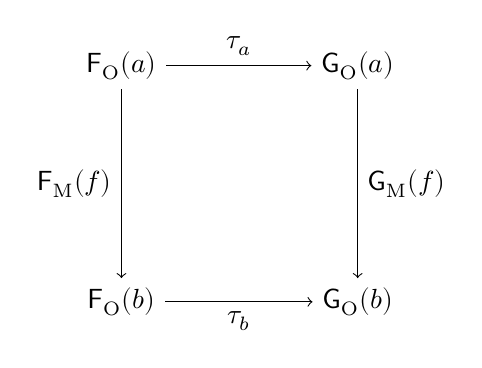
\begin{tikzpicture}[auto,node distance=3cm]
      \node (f a)                {$\funcO{F}(a)$};
      \node (f b) [below of=f a] {$\funcO{F}(b)$};
      \node (g a) [right of=f a] {$\funcO{G}(a)$};
      \node (g b) [below of=g a] {$\funcO{G}(b)$};

      \draw [->] (f a) to node [swap] {$\funcM{F}(f)$}   (f b);
      \draw [->] (g a) to node        {$\funcM{G}(f)$}   (g b);

      \draw [->] (f a) to node        {$\natO{\tau}{a}$} (g a);
      \draw [->] (f b) to node [swap] {$\natO{\tau}{b}$} (g b);
    \end{tikzpicture}
  \end{center}

\end{frame}

%%%%%%%%%%%%%%%%%%%%%%%%%%%%%%%%%%%%%%%%%%%%%%%%%%%%%%%%%%%%%%%%%%%%%%%%%%%%%%

\begin{frame}[fragile]
  \frametitle{Natural Transformations}
  \framesubtitle{Natural Transformations in Haskell}

  \begin{example}
    \begin{code}
head :: [a] -> Maybe a
head []    = Nothing
head (x:_) = x
    \end{code}
  \end{example}

\end{frame}

%%%%%%%%%%%%%%%%%%%%%%%%%%%%%%%%%%%%%%%%%%%%%%%%%%%%%%%%%%%%%%%%%%%%%%%%%%%%%%

\begin{frame}[fragile]
  \frametitle{Natural Transformations}
  \framesubtitle{Natural Transformations in Haskell}

  \begin{example}
    \begin{center}
      \begin{tikzpicture}[auto,node distance=3cm]
        \node (f a)                {|[a]|};
        \node (f b) [below of=f a] {|[b]|};
        \node (g a) [right of=f a] {|Maybe a|};
        \node (g b) [below of=g a] {|Maybe b|};

        \draw [->] (f a) to node [swap] {\UseVerb{fmap f}}   (f b);
        \draw [->] (g a) to node        {\UseVerb{fmap f}}   (g b);

        \draw [->] (f a) to node        {\UseVerb{head}} (g a);
        \draw [->] (f b) to node [swap] {\UseVerb{head}} (g b);
      \end{tikzpicture}
    \end{center}
  \end{example}

\end{frame}

%%%%%%%%%%%%%%%%%%%%%%%%%%%%%%%%%%%%%%%%%%%%%%%%%%%%%%%%%%%%%%%%%%%%%%%%%%%%%%
%%%%%%%%%%%%%%%%%%%%%%%%%%%%%%%%%%%%%%%%%%%%%%%%%%%%%%%%%%%%%%%%%%%%%%%%%%%%%%

\subsection{Monads and Kleisli Triples}

%%%%%%%%%%%%%%%%%%%%%%%%%%%%%%%%%%%%%%%%%%%%%%%%%%%%%%%%%%%%%%%%%%%%%%%%%%%%%%

\begin{frame}
  \frametitle{Monads}

  \begin{definition}[Monad]
    \begin{itemize}
    \item
      Let \cat{C} be a category.
    \item
      A monad $\mon{T} = (\func{T}, \nat{\eta}, \nat{\mu})$ in \cat{C}
      consists of:
      \begin{itemize}
      \item
        An endofunctor $\func{T}: \cat{C} \to \cat{C}$.
      \item
        Natural transformations:
        \begin{itemize}
        \item
          Unit: $\nat{\eta}: \func{I} \to \func{T}: \cat{C} \to
          \cat{C}$
        \item
          Multiplication: $\nat{\mu}: \func{T \comp T} \to \func{T}:
          \cat{C} \to \cat{C}$
        \end{itemize}
      \end{itemize}
    \item
      Such that:
      \begin{itemize}
      \item
        $\natO{\mu}{a} \comp \natO{\mu}{\funcO{T}(a)} = \natO{\mu}{a}
        \comp \funcM{T}(\natO{\mu}{a})$
      \item
        $\natO{\mu}{a} \comp \natO{\eta}{\funcO{T}(a)} =
        \idO{\funcO{T}(a)} = \natO{\mu}{a} \comp
        \funcM{T}(\natO{\eta}{a})$
      \end{itemize}
    \end{itemize}
  \end{definition}

\end{frame}

%%%%%%%%%%%%%%%%%%%%%%%%%%%%%%%%%%%%%%%%%%%%%%%%%%%%%%%%%%%%%%%%%%%%%%%%%%%%%%

\begin{frame}[fragile]
  \frametitle{Monads}
  \framesubtitle{Monads in Haskell}

  \begin{definition}[\UseVerb{Monad'}]
    \begin{code}
class Functor m => Monad' m where
  return :: a -> m a
  join   :: m (m a) -> m a
    \end{code}
  \end{definition}

\end{frame}

%%%%%%%%%%%%%%%%%%%%%%%%%%%%%%%%%%%%%%%%%%%%%%%%%%%%%%%%%%%%%%%%%%%%%%%%%%%%%%

\begin{frame}[fragile]
  \frametitle{Monads}
  \framesubtitle{Monads in Haskell}

  \begin{example}
    \begin{code}
instance Monad' Maybe where
  return :: a -> Maybe a
  return = Just

  join :: Maybe (Maybe a) -> Maybe a
  join Nothing   = Nothing
  join (Just mx) = mx
    \end{code}
  \end{example}

\end{frame}

%%%%%%%%%%%%%%%%%%%%%%%%%%%%%%%%%%%%%%%%%%%%%%%%%%%%%%%%%%%%%%%%%%%%%%%%%%%%%%

\begin{frame}
  \frametitle{Kleisli Triples}

  \begin{definition}[Kleisli triple]
    \begin{itemize}
    \item
      Let \cat{C} be a category.
    \item
      A Kleisli triple $\mon{T} = (\funcO{T}, \nat{\eta},
      \monM{T}{\underscore})$ in $\cat{C}$ consists of:
      \begin{itemize}
      \item
        A natural transformation:
        \begin{itemize}
        \item
          Unit: $\nat{\eta}: \func{I} \to \func{T}: \cat{C} \to
          \cat{C}$
        \end{itemize}
      \end{itemize}
      And assigns:
      \begin{itemize}
      \item
        To each object $a$, an object $\funcO{T}(a)$.
      \item
        To each morphism $f: a \to \funcO{T}(b)$,\\ a morphism
        $\monM{T}{f}: \funcO{T}(a) \to \funcO{T}(b)$.
      \end{itemize}
    \item
      Such that:
      \begin{itemize}
      \item
        $\monM{T}{g} \comp \monM{T}{f} = \monM{T}{(\monM{T}{g} \comp
        f)}$
      \item
        $\monM{T}{f} \comp \natO{\eta}{a} = f$
      \item
        $\monM{T}{\natO{\eta}{a}} = \idO{\funcO{T}(a)}$
      \end{itemize}
    \end{itemize}
  \end{definition}

\end{frame}

%%%%%%%%%%%%%%%%%%%%%%%%%%%%%%%%%%%%%%%%%%%%%%%%%%%%%%%%%%%%%%%%%%%%%%%%%%%%%%

\begin{frame}[fragile]
  \frametitle{Kleisli Triples}
  \framesubtitle{Kleisli Triples in Haskell}

  \begin{definition}[\UseVerb{Monad}]
    \begin{code}
class Monad m where
  return :: a -> m a
  (>>=)  :: m a -> (a -> m b) -> m b

  ...
    \end{code}
  \end{definition}

\end{frame}

%%%%%%%%%%%%%%%%%%%%%%%%%%%%%%%%%%%%%%%%%%%%%%%%%%%%%%%%%%%%%%%%%%%%%%%%%%%%%%

\begin{frame}[fragile]
  \frametitle{Kleisli Triples}
  \framesubtitle{Kleisli Triples in Haskell}

  \begin{definition}[\UseVerb{Monad''}]
    \begin{code}
class Monad'' m where
  return :: a -> m a
  bind   :: (a -> m b) -> m a -> m b
    \end{code}
  \end{definition}

\end{frame}

%%%%%%%%%%%%%%%%%%%%%%%%%%%%%%%%%%%%%%%%%%%%%%%%%%%%%%%%%%%%%%%%%%%%%%%%%%%%%%

\begin{frame}[fragile]
  \frametitle{Kleisli Triples}
  \framesubtitle{Kleisli Triples in Haskell}

  \begin{example}
    \begin{code}
instance Monad'' Maybe where
  return :: a -> Maybe a
  return = Just

  bind :: (a -> Maybe b) -> Maybe a -> Maybe b
  bind _ Nothing  = Nothing
  bind f (Just x) = f x
    \end{code}
  \end{example}

\end{frame}

%%%%%%%%%%%%%%%%%%%%%%%%%%%%%%%%%%%%%%%%%%%%%%%%%%%%%%%%%%%%%%%%%%%%%%%%%%%%%%
%%%%%%%%%%%%%%%%%%%%%%%%%%%%%%%%%%%%%%%%%%%%%%%%%%%%%%%%%%%%%%%%%%%%%%%%%%%%%%

\subsection{Algebras and Initial Algebras}

%%%%%%%%%%%%%%%%%%%%%%%%%%%%%%%%%%%%%%%%%%%%%%%%%%%%%%%%%%%%%%%%%%%%%%%%%%%%%%

\begin{frame}
  \frametitle{Algebras and Initial Algebras}

  \begin{itemize}
  \item
    Let \cat{C} be a category.
  \item
    Let $\func{F}: \cat{C} \to \cat{C}$ be an endofunctor.
  \end{itemize}
  \begin{definition}[Algebra]
    \begin{itemize}
    \item
      An \func{F}-algebra $(a, \alpha)$ is:
      \begin{itemize}
      \item
        An object $a$.
      \item
        A morphism $\alpha: \funcO{F}(a) \to a$.
      \end{itemize}
    \end{itemize}
  \end{definition}

\end{frame}

%%%%%%%%%%%%%%%%%%%%%%%%%%%%%%%%%%%%%%%%%%%%%%%%%%%%%%%%%%%%%%%%%%%%%%%%%%%%%%

\begin{frame}
  \frametitle{Algebras and Initial Algebras}

  \begin{definition}[Algebra homomorphism]
    \begin{itemize}
    \item
      Let $(a,\alpha)$ and $(b,\beta)$ be \func{F}-algebras.
    \item
      An \func{F}-algebra homomorphism $f: (a,\alpha) \to (b,\beta)$
      is a morphism $f: a \to b$ in $\cat{C}$.
    \item
      Such that:
      \begin{itemize}
      \item
        $\beta \comp \funcM{F}(f) = f \comp \alpha$
      \end{itemize}
    \end{itemize}
  \end{definition}

\end{frame}

%%%%%%%%%%%%%%%%%%%%%%%%%%%%%%%%%%%%%%%%%%%%%%%%%%%%%%%%%%%%%%%%%%%%%%%%%%%%%%

\begin{frame}
  \frametitle{Algebras and Initial Algebras}

  \begin{definition}[Algebra homomorphism]
  \end{definition}
  \begin{center}
    \begin{tikzpicture}[auto,node distance=3cm]
      \node (f a)                {$\funcO{F}(a)$};
      \node (a)   [right of=f a] {$a$};
      \node (f b) [below of=f a] {$\funcO{F}(b)$};
      \node (b)   [right of=f b] {$b$};

      \draw [->] (f a) to node        {$\alpha$} (a);
      \draw [->] (f b) to node [swap] {$\beta$}  (b);

      \draw [->] (a)   to node        {$f$}            (b);
      \draw [->] (f a) to node [swap] {$\funcM{F}(f)$} (f b);
    \end{tikzpicture}
  \end{center}

\end{frame}

%%%%%%%%%%%%%%%%%%%%%%%%%%%%%%%%%%%%%%%%%%%%%%%%%%%%%%%%%%%%%%%%%%%%%%%%%%%%%%

\begin{frame}
  \frametitle{Algebras and Initial Algebras}

  \begin{definition}
    \begin{itemize}
    \item
      \func{F}-\alg is the category with:
      \begin{itemize}
      \item
        Objects: \func{F}-algebras.
      \item
        Morphisms: \func{F}-algebra homomorphisms.
      \end{itemize}
    \end{itemize}
  \end{definition}

\end{frame}

%%%%%%%%%%%%%%%%%%%%%%%%%%%%%%%%%%%%%%%%%%%%%%%%%%%%%%%%%%%%%%%%%%%%%%%%%%%%%%

\begin{frame}
  \frametitle{Algebras and Initial Algebras}

  \begin{definition}[Initial algebra]
    \begin{itemize}
    \item
      An \func{F}-algebra $(\mu\func{F},\inmo)$ is the initial
      \func{F}-algebra of \func{F}-\alg if:
      \begin{itemize}
      \item
        For all \func{F}-algebras $(a,\alpha)$, there is a unique
        \func{F}-algebra homomorphism $\cata\alpha:
        (\mu\func{F},\inmo) \to (a,\alpha)$.
      \end{itemize}
      \begin{itemize}
      \item
        That is, a morphism $\cata\alpha: \mu\func{F} \to a$ in
        $\cat{C}$ such that:
        \begin{itemize}
        \item
          $\alpha \comp \funcM{F}(\cata\alpha) = \cata\alpha \comp
          \inmo$
        \end{itemize}
      \end{itemize}
    \end{itemize}
  \end{definition}

\end{frame}

%%%%%%%%%%%%%%%%%%%%%%%%%%%%%%%%%%%%%%%%%%%%%%%%%%%%%%%%%%%%%%%%%%%%%%%%%%%%%%

\begin{frame}
  \frametitle{Algebras and Initial Algebras}

  \begin{definition}[Initial algebra]
  \end{definition}
  \begin{center}
    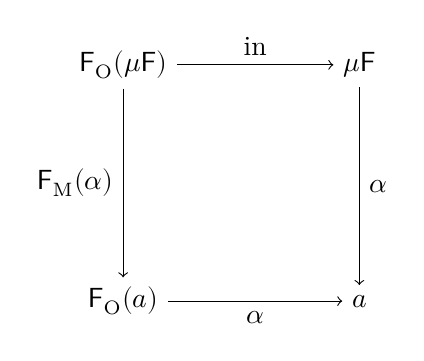
\begin{tikzpicture}[auto,node distance=3cm]
      \node (f a)                {$\funcO{F}(\mu\func{F})$};
      \node (a)   [right of=f a] {$\mu\func{F}$};
      \node (f b) [below of=f a] {$\funcO{F}(a)$};
      \node (b)   [right of=f b] {$a$};

      \draw [->] (f a) to node        {$\inmo$} (a);
      \draw [->] (f b) to node [swap] {$\alpha$}  (b);

      \draw [->] (a)   to node        {$\cata\alpha$}            (b);
      \draw [->] (f a) to node [swap] {$\funcM{F}(\cata\alpha)$} (f b);
    \end{tikzpicture}
  \end{center}

\end{frame}

%%%%%%%%%%%%%%%%%%%%%%%%%%%%%%%%%%%%%%%%%%%%%%%%%%%%%%%%%%%%%%%%%%%%%%%%%%%%%%

\begin{frame}[fragile]
  \frametitle{Algebras and Initial Algebras}
  \framesubtitle{Algebras and Initial Algebras in Haskell}

  \begin{example}
    \begin{code}
data [] a = [] | a : [a]
    \end{code}
    This is an |L|-algebra:
    \begin{code}
data L a b = N | C a b

instance Functor (L a) where
  fmap :: (b -> c) -> L a b -> L a c
  fmap _ N       = N
  fmap g (C x y) = C x (g y)
    \end{code}
  \end{example}

\end{frame}

%%%%%%%%%%%%%%%%%%%%%%%%%%%%%%%%%%%%%%%%%%%%%%%%%%%%%%%%%%%%%%%%%%%%%%%%%%%%%%

\begin{frame}[fragile]
  \frametitle{Algebras and Initial Algebras}
  \framesubtitle{Algebras and Initial Algebras in Haskell}

  \begin{example}
    \begin{code}
data [] a = [] | a : [a]
    \end{code}
    This is the initial |L|-algebra:
    \begin{code}
foldr :: b -> (a -> b -> b) -> [a] -> b
foldr n c []     = n
foldr n c (x:xs) = c x (foldr n c xs)
    \end{code}
  \end{example}

\end{frame}

%%%%%%%%%%%%%%%%%%%%%%%%%%%%%%%%%%%%%%%%%%%%%%%%%%%%%%%%%%%%%%%%%%%%%%%%%%%%%%

\begin{frame}[fragile]
  \frametitle{Algebras and Initial Algebras}
  \framesubtitle{Algebras and Initial Algebras in Haskell}

  \begin{example}
    \begin{code}
(++) :: [a] -> [a] -> [a]
xs ++ ys = (foldr ys (:)) xs
    \end{code}
    \begin{code}
[]     ++ ys = ys
(x:xs) ++ ys = x : xs ++ ys
    \end{code}
  \end{example}

\end{frame}

%%%%%%%%%%%%%%%%%%%%%%%%%%%%%%%%%%%%%%%%%%%%%%%%%%%%%%%%%%%%%%%%%%%%%%%%%%%%%%

\end{document}
